\section{Results}
\label{sec:results}

We now present our comprehensive empirical evaluation of the (closed-source) frontier models on our benchmark for interactive decision-making with long multimodal context.
We investigate how performance changes when presenting more demonstration episodes in the context (see \cref{sec:methods:environments} for a task overview and \cref{app:experimental-details:environments} for details and illustrations).
For each model and task, we first ablate whether to use chain-of-thought prompting and whether to show the legal actions in the prompt (results in \cref{app:additional-results:ablations}).
We use one demonstration episode (\ie still many individual demonstration steps) for these ablations, as a compromise between lower computational demands and being representative of the in-context learning setting.
Due to the very low monthly rate limits of the Anthropic API~\citep{anthropic2024rate}, we do not sweep over the number of demonstrations for \claude{} and only run the ablation.
We also do not evaluate it on Atari since it can only process $100$ images at once (a single demonstration episode hits that limit).

\begin{figure*}[t]
    \begin{center}
        
\includegraphics[width=0.85\textwidth]{figures/main_results}
    \end{center}
    \vspace{-12pt}
    \caption{
        Best scores per model and task across all observation formats, numbers of demonstration episodes, and ablations (chain-of-thought, showing legal actions).
        Accordingly, different bars in a panel may be based on different settings.
        The expert policy (which produced the demonstrations) is an upper baseline.
        The lower baseline randomly selects a legal action at each step.
        \claude{}, \mini{}, and \preview{} cannot be evaluated on Atari -- Phoenix because they cannot process (enough, for \claude{}) images. 
    }
    \label{fig:best-score}
    \vspace{-4pt}
\end{figure*}

\subsection{Best Scores Per Model/Task}
\label{sec:results:best-scores}

\cref{fig:best-score} shows the highest overall score per task and model across all settings (number of demonstrations, observation format, showing legal actions, chain-of-thought prompting).
Different models thus may use different settings on the same task, and the same model may use different settings across tasks. 
In \cref{sec:results:in-context-imitation-learning}, we will keep the observation format and number of demonstrations constant across all models per data point.
As stated above, results for \claude{} are from the ablation (\ie $1$ demonstration episode).
\cref{fig:best-score} shows that models often struggle to match expert scores --- even in their best setting.
Exceptions are grid worlds, which most models largely solve, tic-tac-toe, where the o1 models achieve near-optimal score (against a random opponent), and crosswords, which \preview{} and \oone{} almost solve.
On the other hand, all models always outperform the random action baseline except for Atari -- Phoenix.
LMs tend to repeat actions (see \cref{fig:atari-subsequence-length} for a detailed analysis), and in Phoenix holding down the firing button without releasing results in a single shot (no auto-fire).
In contrast, random actions produce a fair amount of (successful) shots.


\subsection{In-Context Imitation Learning}
\label{sec:results:in-context-imitation-learning}

We now investigate the in-context imitation learning capabilities of today's frontier models, by varying the number of demonstration episodes from zero-, to few-, and many-shot evaluations.
The largest number of demonstrations depends on the models' context sizes, the task, and the tasks' observation formats (images require more tokens than text).
We omit \claude{} due to its low monthly token limit.  

\paragraph{Atari -- Phoenix}

\ificlr
\begin{wrapfigure}{r}{0.5\textwidth}
    \vspace{-20pt}
\else
\begin{figure}[th!]
\fi
    \begin{center}
        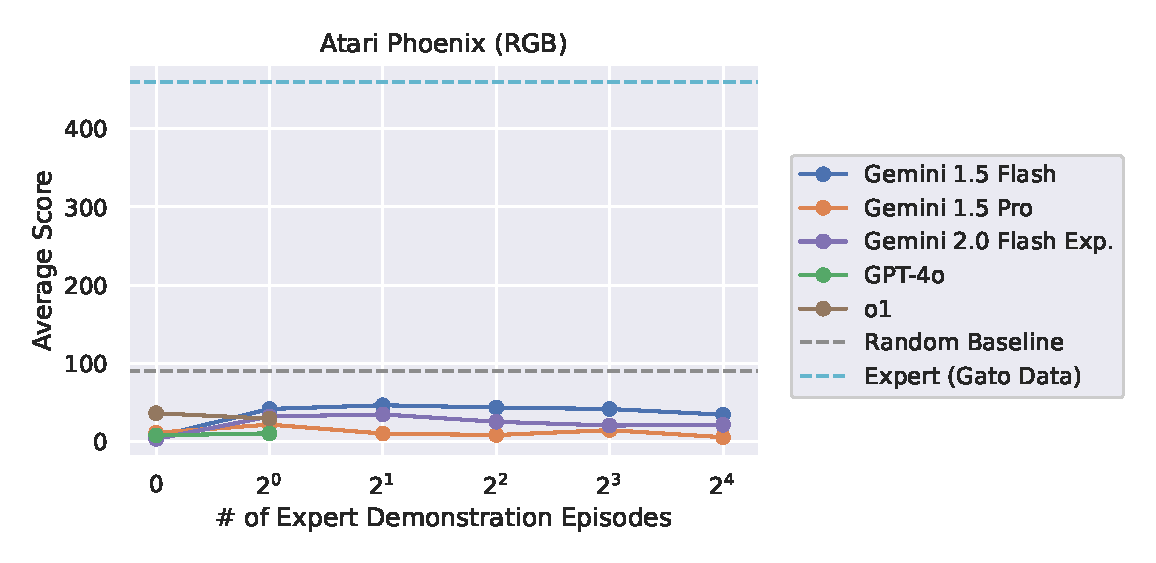
\includegraphics[width=0.5\textwidth]{figures/atari_phoenix_rgb.eps}
    \end{center}
    \vspace{-12pt}
    \caption{
        In-context imitation learning on Atari -- Phoenix (RGB observations).
        Almost all models benefit (mildly) from one demonstration episode, but not from more (\gpt{} and \oone{} cannot fit multiple demonstration episodes in the context).
        While no model outperforms the random baseline, \flash{} performs best.
    }
    \label{fig:atari-phoenix}
    \vspace{-4pt}
\ificlr
\end{wrapfigure}
\else
\end{figure}
\fi

\cref{fig:atari-phoenix} shows that on Atari -- Phoenix all models except \oone{} improve slightly by having one demonstration episode, as opposed none.
However, more demonstrations (only possible for the Gemini models) do not improve the performance further.
All models struggle to outperform the random action baseline because of their tendency to repeat actions (and thus fire very little, since Phoenix has no auto-fire).
\cref{tab:atari-ablation} contains the ablation results.
Models rarely output illegal actions (see \cref{fig:atari-illegal-actions}), \ie they reliably (re)produce the correct action format.
Atari -- Phoenix is arguably the hardest task in our benchmark, since it only comes with image observations (no text representation), and has very large demands \wrt context size (high frame rate, somewhat high resolution images, etc.). 
Despite LMs' massive scale, playing Atari games well (at least by naively feeding raw images to the context) seems currently beyond reach, both in terms of capabilities, but also \wrt context size and compute demands (\cf \citet{waytowich2024atari}).


\ificlr
\begin{figure}
\else
\begin{figure}[th!]
\fi
    \begin{subfigure}[t]{\ificlr0.5\textwidth\else\columnwidth\fi}
        \begin{center}
            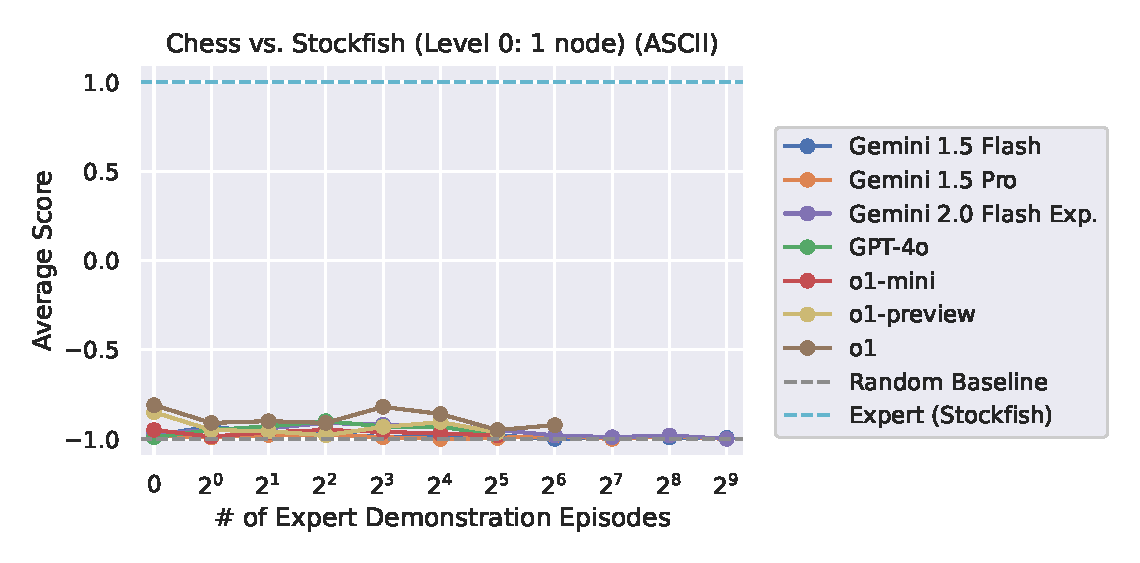
\includegraphics[width=\textwidth]{figures/chess_txt.eps}
        \end{center}
        \vspace{-0.25cm}
        \caption{ASCII observations}
    \end{subfigure}
    \begin{subfigure}[t]{\ificlr0.5\textwidth\else\columnwidth\fi}
        \begin{center}
            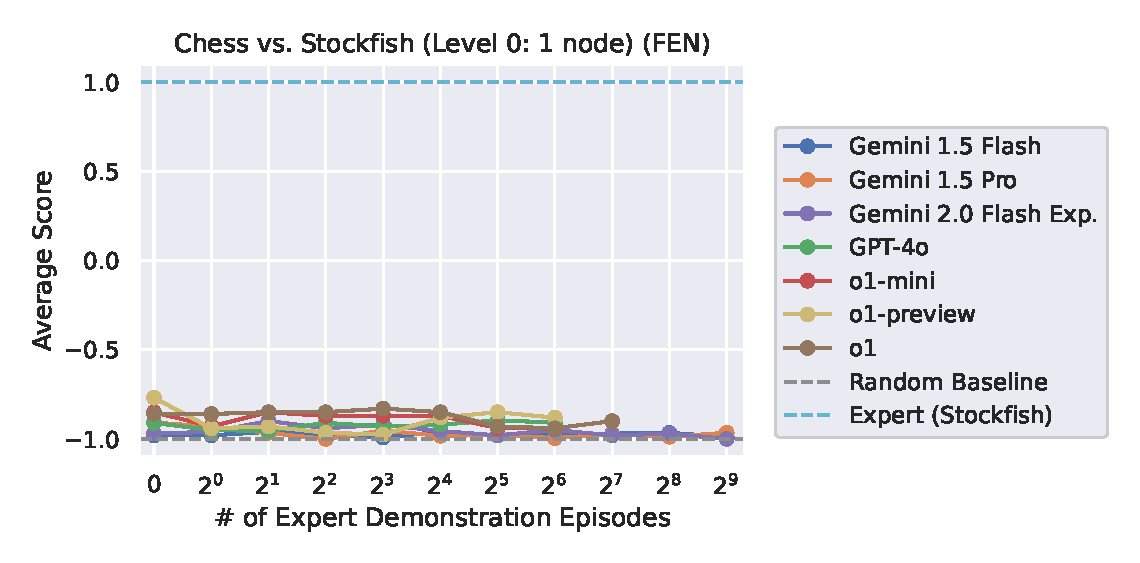
\includegraphics[width=\textwidth]{figures/chess_fen.eps}
        \end{center}
        \vspace{-0.25cm}
        \caption{FEN observations}
    \end{subfigure}
    \begin{subfigure}[t]{\ificlr0.5\textwidth\else\columnwidth\fi}
        \begin{center}
            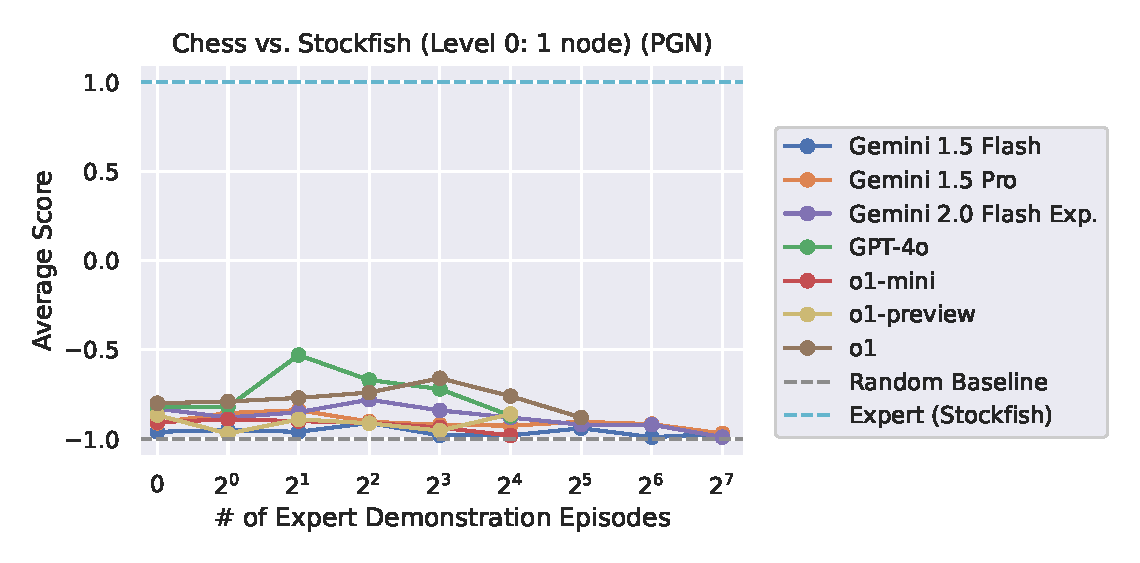
\includegraphics[width=\textwidth]{figures/chess_pgn.eps}
        \end{center}
        \vspace{-0.25cm}
        \caption{PGN observations}
    \end{subfigure}
    \begin{subfigure}[t]{\ificlr0.5\textwidth\else\columnwidth\fi}
        \begin{center}
            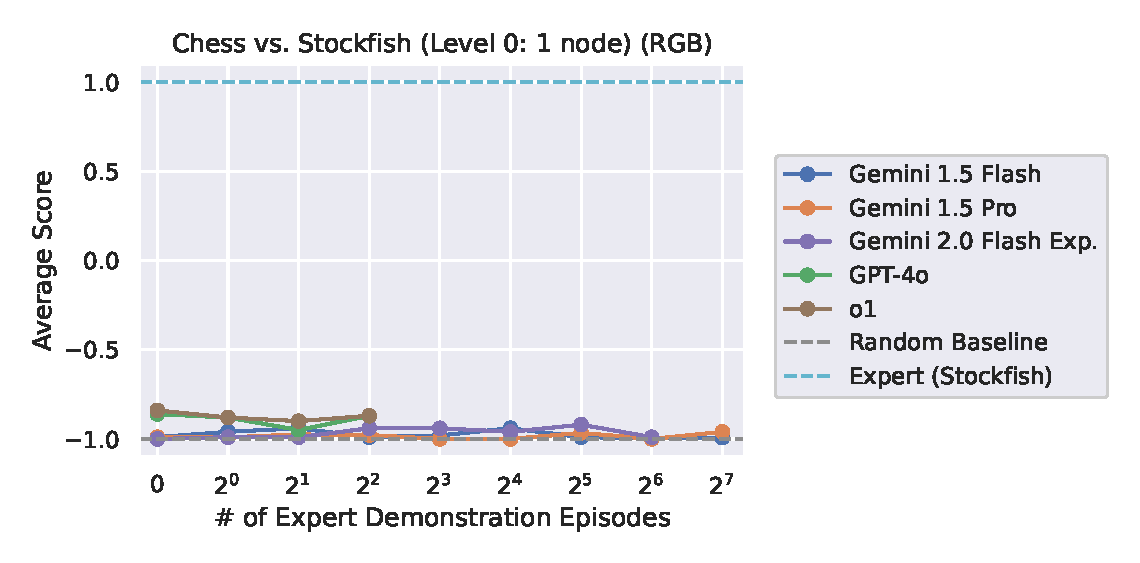
\includegraphics[width=\textwidth]{figures/chess_png.eps}
        \end{center}
        \vspace{-0.25cm}
        \caption{RGB observations}
    \end{subfigure}
    \caption{
        In-context imitation learning on chess against the weakest variant of Stockfish (level $0$, $\approx1300$ Elo), further restricted to one node.
        The models almost always lose (\ie score $-1$) and do not benefit from more demonstrations.
        The PGN observations enable the best results, in particular for \gpt{}, which performs best but still loses majority of games against this weak opponent.
    }
    \vspace{-4pt}
    \label{fig:chess}
\end{figure}

\paragraph{Crosswords}

\ificlr
\begin{wrapfigure}{r}{0.5\textwidth}
    \vspace{-16pt}
\else
\begin{figure}[t]
\fi
   \begin{center}
        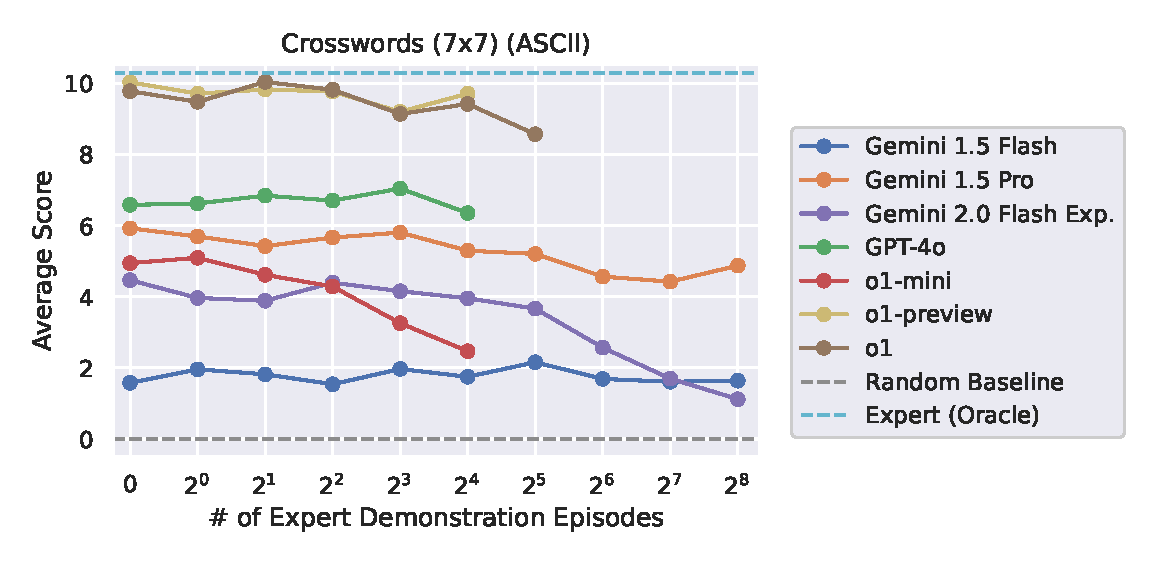
\includegraphics[width=0.5\textwidth]{figures/crossword_txt.eps}
    \end{center}
    \vspace{-8pt}
    \caption{
        In-context imitation learning on $7\times7$ crossword puzzles (using clues with the simplest rating) with ASCII observations.
        The performance of most models is largely unaffected by the number of expert demonstration episodes.
        \preview{} and \oone{} solve most crosswords, while other models struggle to varying degrees.
    }
    \label{fig:crossword}
    \vspace{-4pt}
\ificlr
\end{wrapfigure}
\else
\end{figure}
\fi

\cref{fig:crossword} shows LMs' performance on crosswords with simple clues (as rated by Matthew Ginsberg).
While the models achieve very different overall scores, their individual performance is largely independent of the number of demonstrations (except for \mini{} and \expflash{}, which degrade with more demonstrations).
Overall, \preview{} and \oone{} perform best, almost completely solving all the (simple) crosswords.
\cref{fig:crossword-illegal-actions} shows that the number of illegal actions (\ie where models either suggest a word of incorrect length or fail to respect the ``Across'' \versus ``Down'' format) is quite high for all models and roughly inversely proportional to their puzzle-solving competence.
We use chain-of-thought prompting for some but not all models (see our ablation results in \cref{tab:crossword-ablation}), but we never show the legal actions (which would be a unreasonably long list of words with correct length).

\paragraph{Chess}

\cref{fig:chess} shows LMs' chess-playing performance against the weakest version of Stockfish 16~\citep{romstad2008stockfish}
(\ie level $0$, $\approx1300$ Elo), further restricted to only evaluating a single node.
We investigate four observation formats: ASCII, FEN, PGN, and RGB (\mini{} and \preview{} cannot process images).
Showing more demonstrations has little effect on performance, and models rarely manage to beat (score $1$) or draw (score $0$) against this very weak opponent.
The results show that playing chess (without any scaffolding or fine-tuning) is still out of reach for current LMs.
\cref{fig:chess-illegal-actions} reveals that the models often output illegal actions (which also does not improve with more demonstrations) --- even though the legal actions are provided in the prompt (\cf the ablations in \cref{tab:chess-ablation-anthropic,tab:chess-ablation-gemini,tab:chess-ablation-openai}).

\paragraph{Tic-Tac-Toe}

\begin{figure}
    \begin{subfigure}[t]{0.5\textwidth}
        \begin{center}
            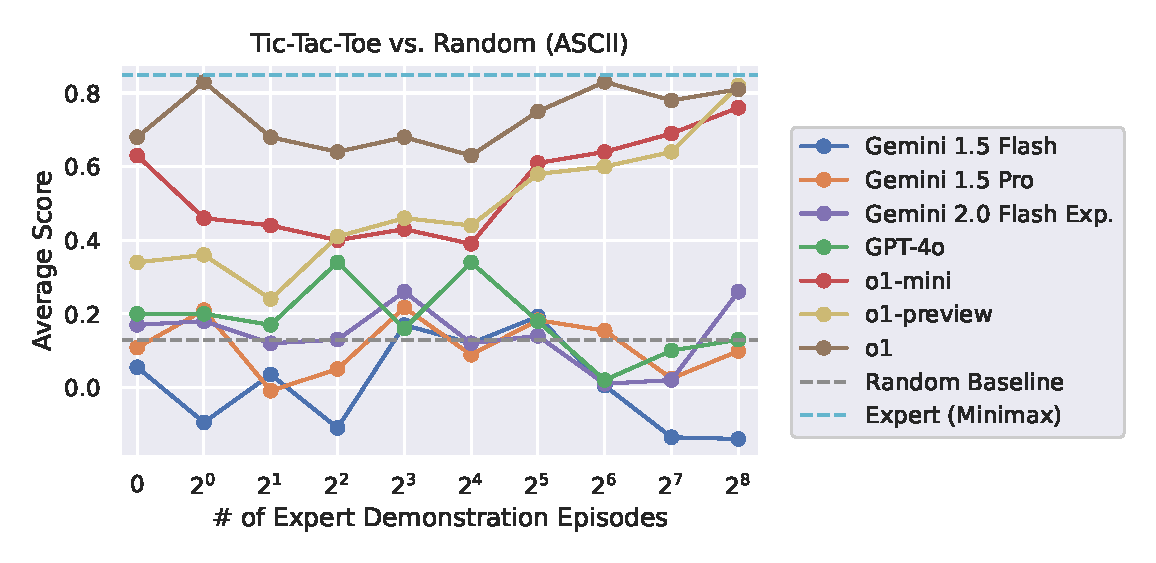
\includegraphics[width=\textwidth]{figures/tic_tac_toe_txt.eps}
        \end{center}
        \vspace{-0.25cm}
        \caption{ASCII observations}
    \end{subfigure}
    \begin{subfigure}[t]{0.5\textwidth}
        \begin{center}
            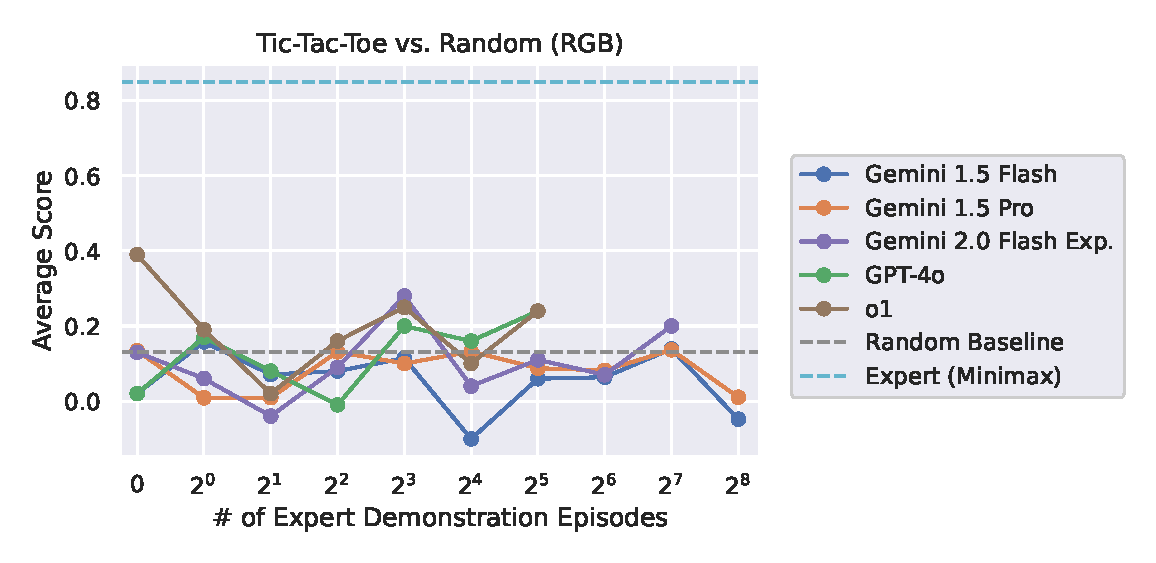
\includegraphics[width=\textwidth]{figures/tic_tac_toe_png.eps}
        \end{center}
        \vspace{-0.25cm}
        \caption{RGB observations}
    \end{subfigure}
    \caption{
        In-context imitation learning on tic-tac-toe against a random action adversary.
        Apart from the o1 models on ASCII observations, all models struggle to play better than a random baseline.
        \mini{} and \preview{} improve with more demonstrations and both reach expert performance at $256$ demonstration episodes.
    }
    \vspace{-4pt}
    \label{fig:tic-tac-toe}
\end{figure}

\cref{fig:tic-tac-toe} shows the results for playing tic-tac-toe against a random-action opponent.
Since the demonstration and evaluation episodes start from different initial states, episodes begin with partially filled boards, which cannot always be won (\ie optimal score $<1$).
The o1 models reach expert performance with ASCII observations and show signs of in-context learning.
The other models struggle to outperform the random action baseline (as does \oone{} with RGB observations).
\cref{fig:tic-tac-toe-illegal-actions} shows that the models (apart from \pro{} on RGB) generate few illegal actions, implying that the models' weak performance is caused by outputting suboptimal rather than illegal actions.

\paragraph{Grid World}

\ificlr
\begin{wrapfigure}{r}{0.5\textwidth}
\vspace{-8pt}
\else
\begin{figure}[th!]
\fi
    \begin{subfigure}[t]{0.5\textwidth}
        \begin{center}
            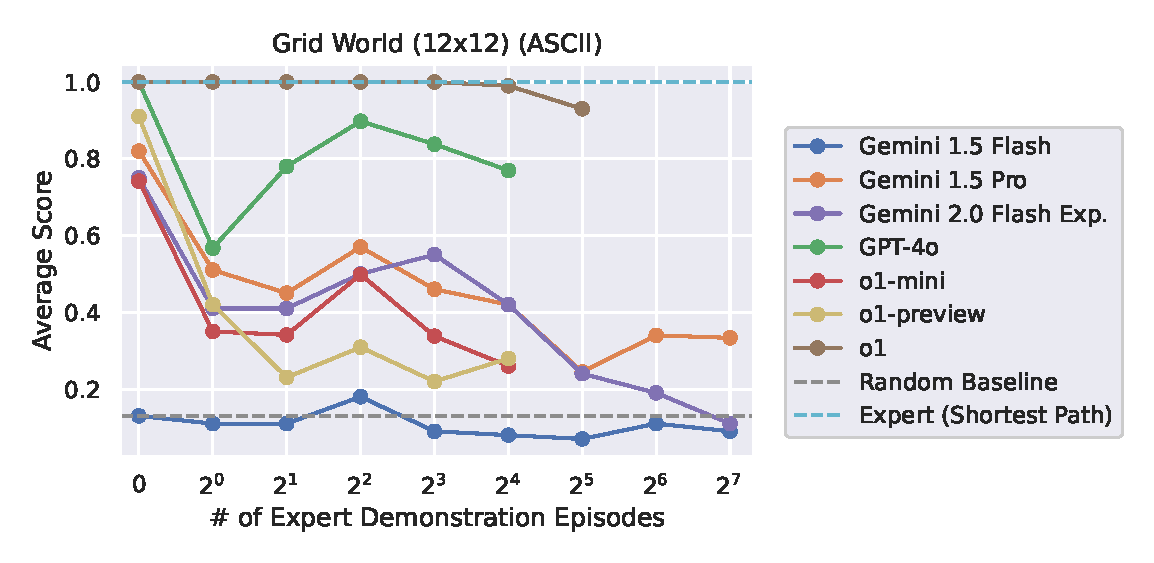
\includegraphics[width=\textwidth]{figures/grid_world_12x12_txt.eps}
        \end{center}
        \vspace{-0.25cm}
        \caption{ASCII observations}
    \end{subfigure}
    \begin{subfigure}[t]{0.5\textwidth}
        \begin{center}
            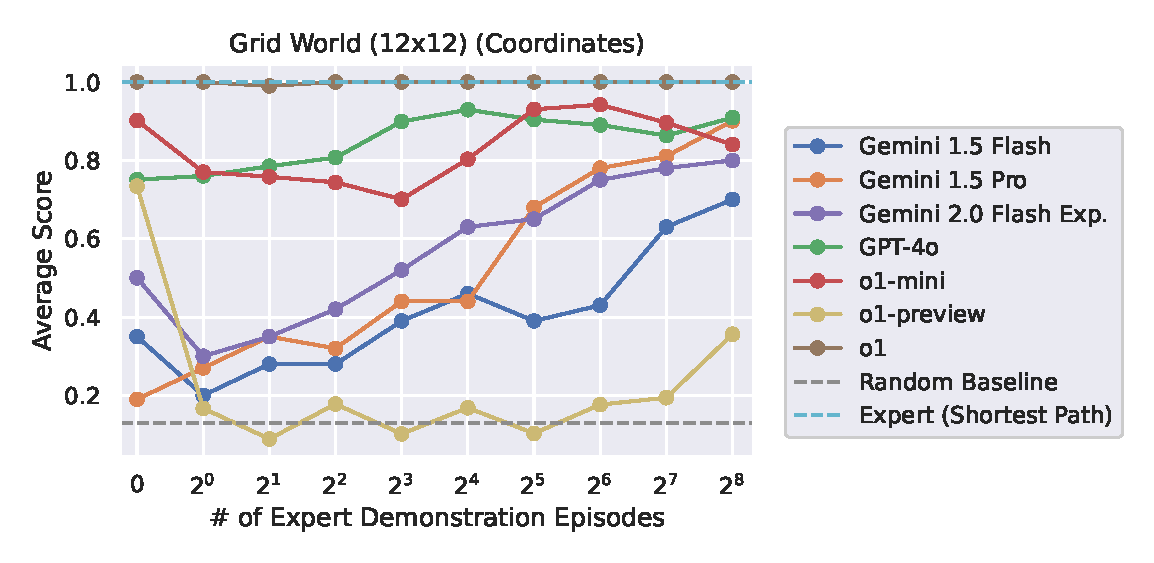
\includegraphics[width=\textwidth]{figures/grid_world_12x12_coords.eps}
        \end{center}
        \vspace{-0.25cm}
        \caption{Coordinate observations}
    \end{subfigure}
    \begin{subfigure}[t]{0.5\textwidth}
        \begin{center}
            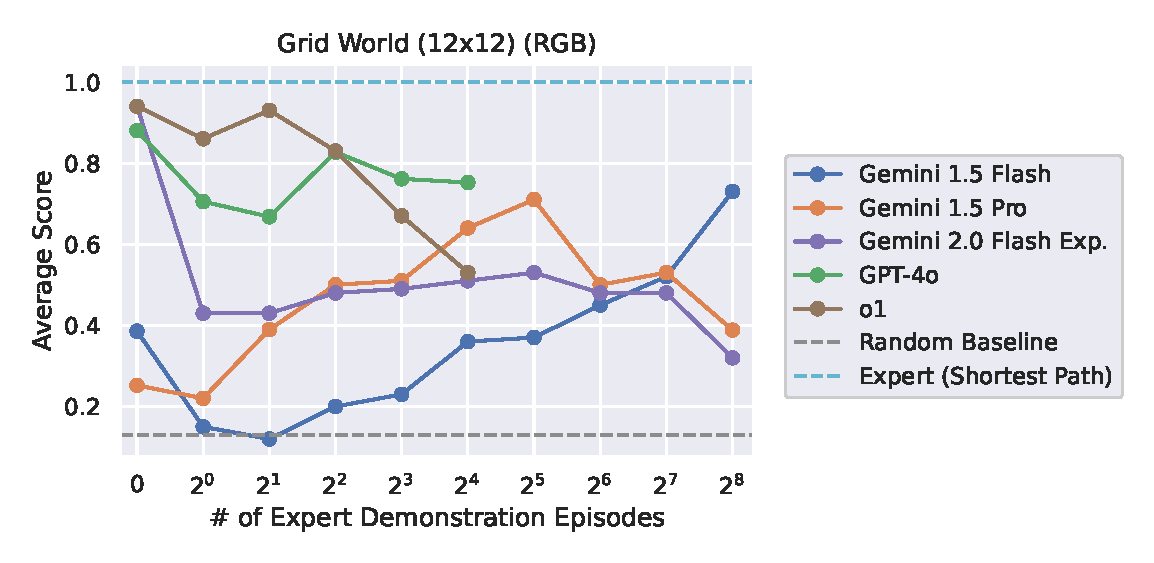
\includegraphics[width=\textwidth]{figures/grid_world_12x12_rgb.eps}
        \end{center}
        \vspace{-0.25cm}
        \caption{RGB observations}
    \end{subfigure}
    \caption{
        In-context imitation learning for navigating to a target in a $12\times12$ grid world (see \cref{fig:observations-grid-world}) using the commands: up, down, left, right.
        On ASCII, most models deteriorate with more demonstrations.
        For coordinate observations (player and target tuple) and RGB images, Gemini improves with more demonstrations (except \expflash{} on RGB), indicating in-context learning across a very long context.
        \gpt{} (and \oone{} on RGB) shows no such a trend but already achieves high zero- and few-shot performance (\oone{} is near-perfect on ASCII and coordinates).
    }
    \label{fig:grid-world}
    \ificlr
    \vspace{-16pt}
    \else
    \vspace{-4pt}
    \fi
\ificlr
\end{wrapfigure}
\else
\end{figure}
\fi

\cref{fig:grid-world} shows how LMs perform on the task of navigating a simple grid world.
The Gemini models steadily improve with more demonstrations for coordinate and RGB image (1.5 models only) observations, demonstrating strong in-context learning with very long contexts.
While \gpt{}, \mini{}, and \preview{} do not benefit from more demonstrations, \oone{} performs very well in almost all settings.
On ASCII observations, most models (except \oone{} and \flash{}) deteriorate with more demonstrations.
\cref{fig:grid-world-illegal-actions} shows the illegal actions for each model, revealing that \preview{}'s performance drops on ASCII and coordinate observations strongly correlate with the number of illegal actions.
All other models rarely generate illegal actions after one demonstration episode.
Overall, grid world is the easiest task in our benchmark where all models perform quite well (some almost optimally) with the right combination of state representation and number of demonstrations.

\paragraph{DM Control -- Cheetah Run}

\cref{fig:dm-control} shows LMs' ability to control a simulated (half) cheetah from DM~Control~\citep{tassa2018deepmind}.
We encode observations and actions as strings (see \cref{fig:observations-dm-control}).
For all models, except \mini{}, a single demonstration episode is helpful but more than two demonstrations degrade performance.
The o1 models struggle to significantly outperform the random action baseline.
\pro{} and \expflash{} achieve the highest score, reaching roughly half the expert score.
Except for \mini{}, all models mostly generate legal actions (see \cref{fig:dm-control-illegal-actions}) --- even without any demonstration episodes (the action format can be inferred from the past actions in the evaluation trajectory since we randomly sample a legal action if the model generates an illegal one).
Therefore, the poor performance in the zero-shot regime (\ie $0$ demonstration episodes) cannot be explained by the models' potential lack of knowledge of the action format.
Instead, models (with the exception of \mini{}) manage to learn a non-trivial policy from one or two demonstration episodes (but fail to leverage more episodes to further improve performance).

